\documentclass[a4paper,10pt]{article}
\usepackage{graphicx}
\usepackage{enumitem}
\usepackage{amsmath}
\usepackage{listings}
\usepackage[usenames,dvipsnames]{color}
\usepackage{bbm}
\usepackage{amsfonts}


%%%%%%%%%%%%%%%%%%%%%%%%%%%%%%%%%%%%%%%%%%%%%%%%%%%%%%%%%%%%%%%%%%%%%%%%%%%%%%%%%%%%%%%%%%%
% MATLAB code listing
%
% This is the color used for MATLAB comments below
\definecolor{MyDarkGreen}{rgb}{0.0,0.4,0.0}
 
% For faster processing, load Matlab syntax for listings
\lstloadlanguages{Matlab}%
\lstset{language=Matlab, % Use MATLAB
frame=single, % Single frame around code
basicstyle=\tiny\ttfamily, % Use small true type font
keywordstyle=[1]\color{Blue}\bfseries, % MATLAB functions bold and blue
keywordstyle=[2]\color{Purple}, % MATLAB function arguments purple
keywordstyle=[3]\color{Blue}\underbar, % User functions underlined and blue
identifierstyle=, % Nothing special about identifiers
% Comments small dark green courier
commentstyle=\usefont{T1}{pcr}{m}{sl}\color{MyDarkGreen}\small,
stringstyle=\color{Purple}, % Strings are purple
showstringspaces=false, % Don't put marks in string spaces
tabsize=5, % 5 spaces per tab
%
%%% Put standard MATLAB functions not included in the default
%%% language here
morekeywords={xlim,ylim,var,alpha,factorial,poissrnd,normpdf,normcdf},
%
%%% Put MATLAB function parameters here
morekeywords=[2]{on, off, interp},
%
%%% Put user defined functions here
morekeywords=[3]{FindESS, homework_example},
%
morecomment=[l][\color{Blue}]{...}, % Line continuation (...) like blue comment
numbers=left, % Line numbers on left
firstnumber=1, % Line numbers start with line 1
numberstyle=\tiny\color{Blue}, % Line numbers are blue
stepnumber=5 % Line numbers go in steps of 5
}
%%%%%%%%%%%%%%%%%%%%%%%%%%%%%%%%%%%%%%%%%%%%%%%%%%%%%%%%%%%%%%%5

\newcommand\scalemath[2]{\scalebox{#1}{\mbox{\ensuremath{\displaystyle #2}}}}

%opening
\title{Determining the Torque Ratings for DC Motors}
\author{Munzir Zafar}

\begin{document}

\maketitle

% \section{Simple Case}
% \begin{figure}[!ht]
% \centering 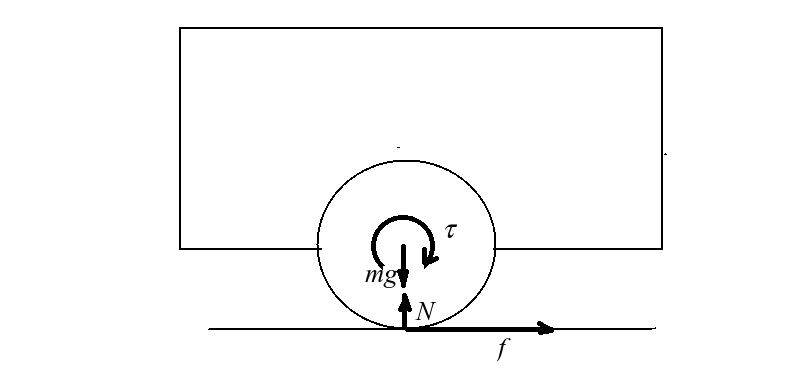
\includegraphics[width=1.0\columnwidth]{Figures/fig1.png}
% \caption{Basic Diagram}
% \label{fig:fig1} 
% \end{figure}
% 
% Summing the horizontal forces:
% \begin{align}
%  f=ma 
% \end{align}
% Summing the vertical forces:
% \begin{align}
%  mg-N=0 
% \end{align}
% Summing Torques:
% \begin{align}
%  \tau-fr = I\alpha
% \end{align}
% Substituting $f$ from first equation:
% \begin{align}
%  \tau-mar=I\alpha \\
%  \tau = mar+I\alpha
% \end{align}

\section{Introduction}

In this report we aim to derive the formula for determining the ratings of the motor needed to be installed on the AGV. 
Special focus is placed on the additional requirements imposed on the motors when AGV is making a turn, in comparison to
when the AGV is moving in a straight line. In order to do this, we will need to derive the dynamic model of the AGV
while it is taking a turn. A dynamic model is the relationship of the forces and torques on a mechanical system with
its speeds, accelerations and its inertial parameters such as masses and inertias. A number of different methods are 
there to determine this dynamic model. We will use Kane's method for the job. 

\section{Turning Dynamics}
\begin{figure}[!ht]
\centering 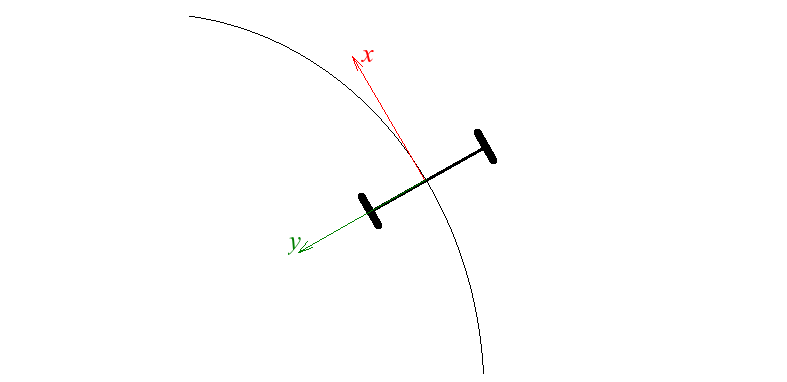
\includegraphics[width=1.0\columnwidth]{Figures/fig2.png}
\caption{Taking a turn}
\label{fig:fig2} 
\end{figure}

Here is a list of symbols used in our derivation:
\begin{itemize}[label={}]
 \item[$\dot{x}$] Forward speed of the AGV
 \item[$\dot\psi$] Rotation speed of AGV 
 \item[$R$] Radius of the wheel
 \item[$L$] Distance between the wheels 
  \item[$\mathbf{MS}_b$] $= \left[\begin{matrix} \mathbf{MX}_b & \mathbf{MY}_b & \mathbf{MZ}_b \end{matrix}\right]^T$ is the center of mass of the AGV body
 \item[$J_b$] $= \left[\begin{matrix} \mathbf{XX}_b & \mathbf{XY}_b & \mathbf{XZ}_b \\ \mathbf{XY}_b & \mathbf{YY}_b & \mathbf{YZ}_b \\ \mathbf{XZ}_b & \mathbf{YZ}_b & \mathbf{ZZ}_b \end{matrix} \right]$ is the inertia matrix of the body
 \item[$J_w$] $= \left[\begin{matrix} \mathbf{XX}_w & 0 & 0 \\ 0 & \mathbf{YY}_w & 0 \\ 0 & 0 & \mathbf{ZZ}_w \end{matrix} \right]$ is the inertia matrix of the wheel
 \item[$\bar{F}$] $= \left[\begin{matrix}  F_x & F_y & F_z  \end{matrix} \right]^T$ is the tugging force (reaction) applied on the AGV
 \item[$E$] $= \left[\begin{matrix}  E_x & E_y & E_z \end{matrix} \right]^T$ are the coordinates of the point at which tugging force is being applied
 \item[$\tau_R, \tau_L$] Torques being applied on right and left wheels
 \item[$\theta_R, \theta_L$] Rotation of right and left wheels
\end{itemize}


\subsection{Defining Generalized Velocities}
% TODO: Explanation of symbols x, psi
It is easier to derive the dynamic model of the system in terms of the generalized velocities:
$\{\dot{q}\} = \{$ $\dot{x}$, $\dot{\psi} \}$. These two velocities can take
arbitrary values all of whom will be kinematically admissible. In other words, they represent
our two degrees of freedom. 
We will now derive two dynamic equations in terms of these generalized velocities. 

Since we are dealing with quasi-velocities, we will use Kane's method to derive the dynamic equations. 

\subsection{Introduction to Kane's formulation}

The Kane's formulation is as follows:
\begin{align}
 \sum_{\substack{k}} \left[ m_k \bar{a}_{Gk} \cdot \left(\bar{v}_{Gk}\right)_j + \left( \frac{d\bar{H}_{Gk}}{dt} 
 \right) \cdot \left( \bar\omega_k \right)_j \right] = \sum_{\substack{n}}  \bar{F}_n \cdot \left( \bar{v}_n \right)_j 
 + \sum_{\substack{n}}  \bar{M}_m \cdot \left( \bar{\omega}_m \right)_j \;\; j=1 ... K \label{kanes}
\end{align}
where 
\begin{itemize}[label={}]
\item[$j$] is the unique number identifying each generalized co-ordinate in the system
\item[$k$] is the unique number identifying each rigid body in the system
\item[$n$] is the unique number identifying each external force acting on the system
\item[$m$] is the unique number identifying each external torque acting on the system
\item[$m_k$] is the mass of the $k$th body
\item[$\bar{a}_{Gk}$] is the acceleration of the center of mass of $k$th body
\item[$\bar{v}_{Gk}$] is the velocity of the center of mass of the $k$th body
\item[$\bar{H}_{Gk}$] is the angular momentum of body $k$ about its center of mass
\item[$\bar{\omega}_{k}$] is the angular velocity of the body $k$
\item[$F_n$] is the $n$th external force
\item[$M_m$] is the $m$th external moment
\item[$\bar{v}_{n}$] is the velocity of the point at which external Force $F_n$ is acting
\item[$\bar{\omega}_{m}$] is the angular velocity of the body on which torque is acting relative to the actuator applying the torque
\item[$()_j$] $=\frac{\partial ()}{\partial \dot{q}_j}$ the partial derivative of the quantity in brackets $()$ with respect to the generalized
velocity $\dot{q}_j$
\end{itemize}

\subsection{Kane's Left-Hand Side}
The left hand side of the Kane's equation containes a sum whose range is equal to the number of bodies
in the system. We have three bodies: Left-wheel ($L$), right wheel ($R$) and the body of robot ($B$). 
Each term in the sum consists of the acceleration ($\bar{a}_{Gk}$), velocity ($\bar{v}_{Gk}$), 
angular momentum ($\bar{H}_{Gk}$) of the center of mass and the body's angular velocity ($\bar{\omega}_k$). 
And then some partieal derivatives wrt to the generalized coordinates 
($(\bar{\omega}_k)_j=\frac{\partial \bar{\omega}_k}{\partial \dot{q}_j}$ and 
$(\bar{v}_{Gk})_j=\frac{\partial \bar{v}_{Gk}}{\partial \dot{q}_j}$). We will have two equations 
corresponding to each generalized coordinate $\{\dot{q}_j\} = \{$ $\dot{x}$, $\dot{\psi} \}$.

\subsubsection{Left Wheel}
% TODO: Figure explaining the co-ordinate frames missing
% TODO: The relationships of thetaL with xdot and psidot missing
This evaluation takes place in the $x_Ly_Lz_L$ frame fixed to the left wheel such that it is parallel to 
frame $x_0y_0z_0$ when $\theta_L = 0$. So $\bar{i}_0 = cos\theta_L\bar{i}_L+sin\theta_L\bar{k}_L$, 
$\bar{j}_0 = \bar{j}_L$ and $\bar{k}_0 = -sin\theta_L\bar{i}_L+cos\theta_L\bar{k}_L$.
Angular velocity:
\begin{align}
 \bar{\omega}_L &= \dot\psi\bar{k}_0 + \dot\theta_L\bar{j_0} \nonumber \\
 &= \dot\psi\bar{k}_0 + \left(\frac{1}{R}\dot{x}-\frac{L}{2R}\dot\psi\right)\bar{j}_0 \nonumber \\
 &= -\dot\psi sin\theta_L\bar{i}_L + \left(\frac{1}{R}\dot{x}-\frac{L}{2R}\dot\psi\right)\bar{j}_L + \dot\psi cos\theta_L\bar{k}_L \label{kanesLHSVariableStart}
\end{align}
The terms that follow are also similarly to be expressed in frame $x_Ly_Lz_L$ but that step is skipped for brevity.
Velocity:
\begin{align}
  \bar{v}_{GL} &= \bar{v}_0 + \bar{\omega}_0 \times \bar{r}_{L/O} \nonumber \\
 &= \dot{x}\bar{i}_0 + \dot\psi\bar{k}_0 \times \frac{L}{2}\bar{j}_0 \nonumber \\
 &= \left(\dot{x}-\frac{L}{2}\dot\psi\right)\bar{i}_0  
\end{align}
Linear acceleration:
\begin{align}
 \bar{a}_{GL} &= \bar{a}_0 + \bar\alpha_0 \times \bar{r}_{L/O} + \bar\omega_0 \times \left( \omega_0 \times \bar{r}_{L/O}\right) \nonumber \\
 &= \ddot{x}\bar{i}_0 + \dot{x}\left(\dot\psi\bar{k}_0 \times \bar{i}_0\right)+ \ddot\psi\bar{k}_0 \times \frac{L}{2}\bar{j}_0 + \dot\psi\bar{k}_0 \times \left( \dot\psi\bar{k}_0 \times \frac{L}{2}\bar{j}_0\right) \nonumber \\
 &= \left(\ddot{x}-\frac{L}{2}\ddot\psi\right)\bar{i}_0 + \left(\dot{x}\dot\psi- \frac{L}{2}\dot\psi^2\right)\bar{j}_0  
\end{align}
Angular momentum and its derivative:
\begin{align}
 \bar{H}_{GL} &= I_w\bar{\omega}_L \nonumber \\
 \frac{d\bar{H}_{GL}}{dt} &= \frac{\partial \bar{H}_{GL}}{\partial t} + \bar\omega_L \times \bar{H}_{GL} \nonumber \\
\end{align}
where $I_w = \scalemath{0.75}{\left[\begin{matrix} \mathbf{ZZ}_w & 0 & 0 \\  0 & \mathbf{YY}_w & 0 \\ 0 & 0 & \mathbf{ZZ}_w \end{matrix}\right]}$. Due to symmetry the off-diogonal terms in the inertia matrix vanish, and the 
inertia about $x_L$-axis and $z_L$-axis are both equal (signified by $\mathbf{ZZ}_w$).

\subsubsection{Right Wheel}
This evaluation takes place in the $x_Ry_Rz_R$ frame fixed to the right wheel such that it is parallel to 
frame $x_0y_0z_0$ when $\theta_R = 0$. So $\bar{i}_0 = cos\theta_R\bar{i}_R+sin\theta_R\bar{k}_R$, 
$\bar{j}_0 = \bar{j}_R$ and $\bar{k}_0 = -sin\theta_R\bar{i}_R+cos\theta_R\bar{k}_R$.
Angular velocity:
\begin{align}
 \bar{\omega}_R &= \dot\psi\bar{k}_0 + \dot\theta_R\bar{j_0} \nonumber \\
 &= \dot\psi\bar{k}_0 + \left(\frac{1}{R}\dot{x}+\frac{L}{2R}\dot\psi\right)\bar{j}_0 \nonumber \\
 &= -\dot\psi sin\theta_L\bar{i}_R + \left(\frac{1}{R}\dot{x}+\frac{L}{2R}\dot\psi\right)\bar{j}_R + \dot\psi cos\theta_L\bar{k}_R 
\end{align}
The terms that follow are also similarly to be expressed in frame $x_Ry_Rz_R$ but that step is skipped for brevity.
Velocity:
\begin{align}
  \bar{v}_{GR} &= \bar{v}_0 + \bar{\omega}_0 \times \bar{r}_{R/O} \nonumber \\
 &= \dot{x}\bar{i}_0 + \dot\psi\bar{k}_0 \times \left(-\frac{L}{2}\bar{j}_0\right) \nonumber \\
 &= \left(\dot{x}+\frac{L}{2}\dot\psi\right)\bar{i}_0  
\end{align}
Linear acceleration:
\begin{align}
 \bar{a}_{GR} &= \bar{a}_0 + \bar\alpha_0 \times \bar{r}_{R/O} + \bar\omega_0 \times \left( \omega_0 \times \bar{r}_{R/O}\right) \nonumber \\
 &= \ddot{x}\bar{i}_0 + \dot{x}\left(\dot\psi\bar{k}_0 \times \bar{i}_0\right)+ \ddot\psi\bar{k}_0 \times \left(-\frac{L}{2}\bar{j}_0\right) + \dot\psi\bar{k}_0 \times \left( \dot\psi\bar{k}_0 \times \left(-\frac{L}{2}\bar{j}_0\right)\right) \nonumber \\
 &= \left(\ddot{x}+\frac{L}{2}\ddot\psi\right)\bar{i}_0 + \left(\dot{x}\dot\psi + \frac{L}{2}\dot\psi^2\right)\bar{j}_0  
\end{align}
Angular momentum and its derivative:
\begin{align}
 \bar{H}_{GR} &= I_w\bar{\omega}_R \nonumber \\
 \frac{d\bar{H}_{GR}}{dt} &= \frac{\partial \bar{H}_{GR}}{\partial t} + \bar\omega_0 \times \bar{H}_{GR} \nonumber \\
\end{align}

\subsubsection{Body}
We will evaluate the quantities in frame $x_0y_0z_0$. \\
Angular velocity:
\begin{align}
 \bar{\omega}_B &= \dot\psi\bar{k}_0 
\end{align}
\\Velocity:
\begin{align}
  \bar{v}_{GB} &= \bar{v}_0 + \bar{\omega}_B \times \bar{r}_{B/O} \nonumber \\
  &= \dot{x}\bar{i}_0 + \bar{\omega}_B \times \frac{1}{m_B}\mathbf{MS}_{B} 
\end{align}isa
Linear acceleration:
\begin{align}
 \bar{a}_{GB} &= \bar{a}_0 + \bar\alpha_B \times \bar{r}_{B/O} + \bar\omega_B \times \left( \bar\omega_B \times \bar{r}_{B/O}\right) 
\end{align}
where 
\begin{align} \begin{split}
 &\bar{a}_0 = \frac{d\bar{v}_0}{dt} = \frac{d\left(\dot{x}\bar{i}_0\right)}{dt} 
 = \ddot{x}\bar{i}_0+\dot{x}\left(\dot\psi\bar{k}_0 \times \bar{i}_0\right)  \\
 &\bar\alpha_B = \frac{d\bar{\omega}_B}{dt} = \frac{d\left(\dot\psi\bar{k}_0 \right)}{dt}
 = \ddot\psi\bar{k}_0  \label{a0alphaB}
\end{split} \end{align}
Angular momentum and its derivative:
\begin{align}
 \bar{H}_{GB} &= I_B\bar{\omega}_B \nonumber \\
 \frac{d\bar{H}_{GB}}{dt} &= \frac{\partial \bar{H}_{GB}}{\partial t} + \bar\omega_B \times \bar{H}_{GB} \label{kanesLHSVariableEnd}
\end{align}

\subsubsection{Left-Hand Side Final Evaluation}
The Kanes' formulation (Eq. \ref{kanes}) are in fact two equations each corresponding to a different generalized velocity
${\dot{q}_j} = {\dot{x},\dot\psi}$. Each of these three equation is a summation of the given expression evaluated
for each body ${k}={L,R,B}$ i.e. Left-wheel, right-wheel and body. When the expressions that we evaluated in eqs. 
\ref{kanesLHSVariableStart}-\ref{kanesLHSVariableEnd} are substituted in Kanes' equations (Eq. \ref{kanes}) and the results 
evaluted (using MATLAB code listed in the Appendix section \ref{app1}), we get the following expression:
\begin{align}
 &\mathbf{A\ddot{q}+C\dot{q}} \nonumber
\end{align}\\
where
\begin{align} \begin{split}
 &\mathbf{A}=\scalemath{0.75}{\left[\begin{matrix}
  m_B+2m_w+\frac{2\mathbf{YY}_w}{R^2} &
  -\mathbf{MY}_b \\
  -\mathbf{MY}_b &
  \frac{m_wL^2}{2}+\frac{\mathbf{YY}_wL^2}{2R^2}+2\mathbf{ZZ}_w + \frac{\mathbf{MX}_b^2}{m_B} + \frac{\mathbf{MY}_b^2}{m_b}  + \mathbf{ZZ}_b\\
  \end{matrix}\right]}  \\
 &\mathbf{C}=\scalemath{0.75}{\left[\begin{matrix}
  0 &
  -\mathbf{MX}_b\dot\psi \\
  \frac{1}{2}\mathbf{MX}_b\dot\psi &  
  \frac{1}{2}\mathbf{MX}_b\dot{x} \\
 \end{matrix}\right]} \label{kanesAC}
\end{split}\end{align}

\subsection{Kane's Right Hand Side}

The right hand side of the Kane's forumulation \ref{kanes} is the sum of some dot product terms. Each term is either the
dot product of:
\begin{itemize}
 \item force applied on the system $\bar{F}_n$
 \item the linear velocity $\bar{v}_n$ of the point differentiated partially wrt the the unique gerneralized speed 
 $\dot{q}_j$ corresponding to each equation i.e. $\frac{\partial \bar{v}_n}{\partial \dot{q}_j}$\\
\end{itemize}
or the dot product of:
\begin{itemize}
 \item torque applied on the system $\bar{\tau}_n$
 \item the angular velocity $\bar{\omega}_n$ of the body differentiated partially wrt the the unique gerneralized speed 
 $\dot{q}_j$ corresponding to each equation i.e. $\frac{\partial \bar{\omega}_n}{\partial \dot{q}_j}$
\end{itemize}

So, in order to analyse the right-hand side of the equation, we need to list down all the forces and torques applied
to the system and the points at which they are being applied. They are as follows:
\begin{itemize}[label={}]
 \item[$\bar\tau_L, \bar\tau_R $] Torques applied by wheel motors (in the body) on the right wheel and left wheel at points 
 $R$ and $L$ on the respective wheels
 \item[$\bar{F}$] The reaction force from the load being tugged by the AVG acting at point $E$
\end{itemize}

Let $\scalemath{0.75}{\bar{F} = \left[\begin{matrix} F_{x} & F_{y} & F_{z} \end{matrix}\right]^T}$
be the components of forces/torques defined in the frame $x_0y_0z_0$ and $\scalemath{0.75}{\bar{r}_{E/O} = \left[\begin{matrix} -E_x & 0 & E_z \end{matrix}\right]^T}$ are the
coordinates of point $E$ in the $x_0y_0z_0$ frame. Also 
$\scalemath{0.75}{\bar{F}_{g} = \left[\begin{matrix} 0 & 0 & -m_bg \end{matrix}\right]^T}$.
Also $\bar{r}_{G/O}$ is to be expressed in the $x_0y_0z_0$ which will be
$\scalemath{0.75}{\bar{r}_{G/O} = \frac{1}{m_B} \left[\begin{matrix} \mathbf{MX}_{B} \\ \mathbf{MY}_{B} \\ \mathbf{MZ}_{B} \end{matrix}\right]}$.

\vspace{5mm}

We now give closed form expressions of terms contributed on the RHS by these forces and torques:

\vspace{5mm} 
\begin{enumerate}
 \item Torque on the wheel at $L$ will contribute the following terms
\begin{align}
 & \tau_L\bar{j}_0 \cdot \frac{\partial \bar{\omega}_L}{\partial \dot{q}_j}
\end{align}
where $\bar{\omega}_L = \dot\psi\bar{k}_0 + \left(\frac{1}{R}\dot{x}-\frac{L}{2R}\dot\psi\right)\bar{j}_0$

\vspace{5mm}

 \item Torque on the wheel at $R$ will contribute the following terms
\begin{align}
 & \tau_R\bar{j}_0 \cdot \frac{\partial \bar{\omega}_R}{\partial \dot{q}_j}
\end{align}
where $\bar{\omega}_R = \dot\psi\bar{k}_0 + \left(\frac{1}{R}\dot{x}+\frac{L}{2R}\dot\psi\right)\bar{j}_0$

\vspace{5mm}
 \item The force $\bar{F}$ contributes the following term:
\begin{align}
 & \bar{F} \cdot \frac{\partial \bar{v}_E}{\partial \dot{q}_j}
\end{align}
where 
\begin{align}
 \bar{v}_E &= \bar{v}_0 + \bar\omega_B \times \bar{r}_{E/O} \nonumber \\
 &= \dot{x}\bar{i}_0 + \dot\psi\bar{k}_0 \times \left( -E_x\bar{i}_0 + E_z\bar{k}_0 \right) \nonumber \\
 &= \dot{x}\bar{i}_0 - E_x\dot\psi\bar{j}_0
\end{align}
\end{enumerate}

The overall contribution of the forces and torques on the right-hand side of the Kane's equations is:
\begin{itemize}[label={}]
 \item[$\dot{x}$:]  $\frac{1}{R}\left(\tau_R + \tau_L\right) + F_x$
 \item[$\dot\psi$:] $\frac{L}{2R}\left(\tau_R-\tau_L\right) - E_xF_y$
\end{itemize}

\subsection{Final Expression for the Turning Dynamics}
\begin{align}
  \scalemath{0.75}{\left(m_B+2m_w+\frac{2\mathbf{YY}_w}{R^2}\right)\ddot{x} - \mathbf{MY}_b\ddot\psi -\mathbf{MX}_b\dot\psi^2} &\scalemath{0.75}{= \frac{1}{R}\left(\tau_R + \tau_L\right) + F_x} \label{dyn1}\\
  \scalemath{0.75}{-\mathbf{MY}_b\ddot{x} + \left(\frac{m_wL^2}{2}+\frac{\mathbf{YY}_wL^2}{2R^2}+2\mathbf{ZZ}_w + \frac{\mathbf{MX}_b^2}{m_B} + \frac{\mathbf{MY}_b^2}{m_b}  + \mathbf{ZZ}_b\right)\ddot\psi + \mathbf{MX}_b\dot{x}\dot\psi} &= \scalemath{0.75}{\frac{L}{2R}\left(\tau_R-\tau_L\right) - E_xF_y} \label{dyn2}
\end{align}

\section{Torque Requirements}
The dynamic equation \ref{dyn1}-\ref{dyn2} can be used to find out expressions for $\tau_R$ and $\tau_L$. We get:
% dyn1LHS*R-Fx = tR+tL
% dyn2LHS*2R/L+ExFy = tR-tL
% tR = (dyn1LHS*R-Fx + dyn2LHS*2R/L+ExFy)/2
% tL = (dyn1LHS*R-Fx - dyn2LHS*2R/L-ExFy)/2
\begin{align}
 \scalemath{0.75}{\tau_R} & \scalemath{0.75}{=\left(\mathbb{M}_1-\frac{R}{L}\mathbf{MY}_b\right)\ddot{x} + \left(-\frac{R}{2}\mathbf{MY}_b+\mathbb{M}_2\right)\ddot\psi - \frac{R}{2}\mathbf{MX}_b\dot\psi^2 + \frac{R}{L}\mathbf{MX}_b\dot{x}\dot\psi - \frac{R}{2}F_x + \frac{R}{L}E_xF_y} \\
 \scalemath{0.75}{\tau_L} & \scalemath{0.75}{=\left(\mathbb{M}_1+\frac{R}{L}\mathbf{MY}_b\right)\ddot{x} + \left(-\frac{R}{2}\mathbf{MY}_b-\mathbb{M}_2\right)\ddot\psi - \frac{R}{2}\mathbf{MX}_b\dot\psi^2 - \frac{R}{L}\mathbf{MX}_b\dot{x}\dot\psi - \frac{R}{2}F_x - \frac{R}{L}E_xF_y} 
\end{align}where
\begin{align}
 \scalemath{0.75}{\mathbb{M}_1} &= \scalemath{0.75}{\frac{R}{2}\left(m_B+2m_w+\frac{2\mathbf{YY}_w}{R^2}\right)} \label{M1} \\
 \scalemath{0.75}{\mathbb{M}_2} &= \scalemath{0.75}{\frac{R}{L}\left(\frac{m_wL^2}{2}+\frac{\mathbf{YY}_wL^2}{2R^2}+2\mathbf{ZZ}_w + \frac{\mathbf{MX}_b^2}{m_B} + \frac{\mathbf{MY}_b^2}{m_b}  + \mathbf{ZZ}_b\right)} \label{M2}
\end{align}

If the mass distribution of the AGV body is symmetrical then $\mathbf{MX}_b = \mathbf{MY}_b = 0$ then:
\begin{align}
 \tau_R &= \mathbb{M}_1\ddot{x} + \mathbb{M}_2\ddot\psi - \frac{R}{2}F_x + \frac{R}{L}E_xF_y \label{turning1} \\
 \tau_L &= \mathbb{M}_1\ddot{x} - \mathbb{M}_2\ddot\psi - \frac{R}{2}F_x - \frac{R}{L}E_xF_y  \label{turning2}
\end{align}

If the system is moving on a straight path then there is no rotation of the body about its center $\dot\psi = \ddot\psi = 0$ and the 
y-component of the tug force is also zero meaning $F_y = 0$. The equations become:
\begin{align}
 \tau_R &= \mathbb{M}_1\ddot{x} - \frac{R}{2}F_x \label{straight1} \\
 \tau_L &= \mathbb{M}_1\ddot{x} - \frac{R}{2}F_x \label{straight2}
\end{align}

In order to estimate toque limits, let's insert estimates of various parameters that appear in the above equations:
\begin{align}
 R &= 20 in = 10 \times 0.0254 = 0.254 m \nonumber \\
 \mathbb{M}_1 &= \frac{R}{2} \times 300 kg =  38.1 kgm \nonumber \\
 \ddot{x}_{max} &= \frac{18 m/min}{1 s} = 0.3 m/s^2 \nonumber \\
 F_x &= 1000 kg \times 0.3 m/s^2 = 300 N \nonumber \\
 L &= 3 ft = 0.9 m \nonumber \\
 W &= 4 ft = 1.2 m \nonumber \\
 \mathbf{ZZ}_b &= \frac{1}{12}m_b\left(L^2+W^2\right) = \frac{1}{12}\times 300 \left(1.2^2+0.9^2\right) = 56.25 kgm^2 \nonumber \\
 \mathbb{M}_2 &= \frac{R}{L}\mathbf{ZZ}_b = 15.625 kgm^2 \nonumber \\
 \ddot\psi_{max} &= 15 rad/s^2 \nonumber \\
 \tau_{straight} &= 49.53 Nm \nonumber \\
 P_{straight} &= \tau_{straight} \frac{\dot{x}_{max}}{R} = 58.5 Watts \nonumber \\
 \tau_{turning} &= 234.37 Nm \nonumber \\
 P_{turning} &= \tau_{turning} \frac{\dot{x}_{max}}{R} = 276.82 Watts \nonumber 
\end{align}


\section{Conclusion}

Equations \ref{turning1}-\ref{turning2} represent dynamics while the robot is turning, while equations \ref{straight1}-\ref{straight2} 
represent dynamics while the robot is moving in a straight line. Upon comparison it is clear that there are two additional terms 
in the turning motion which will increase the torque requirements of the robot: $\frac{1}{2}E_xF_y$ and $\mathbb{M}_2\ddot\psi$.
The first of these two terms is simply the torque exerted by the load being tugged. To analyse the second term however, we will need to 
look at the definition of $\mathbb{M}_2$ in eq. \ref{M2}. The most dominant term defining 
$\mathbb{M}_2$ (eq. \ref{M2}) is $\mathbf{ZZ}_b$ i.e. the inertia of the AGV body about vertical (or $z$-) axis. 
This is because the rest of the terms are either zero ($\mathbf{MX}_b, \mathbf{MY}_b$) or small in comparison 
($m_w, \mathbf{YY}_w$). This inertia terms ($\mathbf{ZZ}_b$) is multiplying with rotational accelration of the body about the vertical ($\ddot\psi$).
Now, as the AGV encounters a turn in its path, this rotational acceleration jumps from zero to a positive value. And the second term 
comes into play. The control algorithm should try to minimize this acceleration in order to minimize this term. 


\appendix

\section{MATLAB code for Evaluation of Kane's Equaiton}

\subsection{Kane's LHS} 

This is the code listing for the evaluation of Kane's equation LHS (Eq. \ref{kanes}) for our robot:
\lstinputlisting[language=Matlab]{../matlab/dynamicsLHS.m}

\subsection{Kane's RHS} 

This is the code listing for the evaluation of Kane's equation RHS (Eq. \ref{kanes}) for our robot:
\lstinputlisting[language=Matlab]{../matlab/dynamicsRHS.m}


\end{document}
